
\subsection{Andamento sistema del terzo ordine}
Si consideri una matrice della dinamica del seguente tipo
$$
A = \begin{pmatrix}
-3 & 3 & 0\\
-2 & 3 & 2\\
0  & -6 & -3
\end{pmatrix}
$$
lo stato iniziale del sistema è
$$
x_0 = (1 \ 1\ 1)^T
$$
Si ricavano gli autovalori e gli autovettori risolvendo il polinomio
caratteristico
$$
\left\{\begin{aligned}
\lambda &= -3 &\rightarrow& u^T=(1, 0, 1)\\
\alpha &\pm j\omega = \pm j3 &\rightarrow& u_a^T=(-1, -1 , 2),\ u_b^T = (0, -1 ,
0)
\end{aligned}\right.
$$

Si deve successivamente operare una trasformazione di coordinate
$$
Z = U_r^{-1}x = (u\ u_a \ u_b)^{-1}x
$$
la risposta libera sarà
$$
x_l = U_re^{\Lambda_r t}U_r^{-1} x_0 = U_r e^{\Lambda_r t} z_0
$$
dato che $z = U_r^{-1} x$

Si rappresenta la traiettoria dello stato nello spazio $z$

\begin{figure}[H]
 \centering
 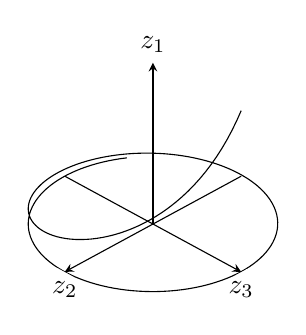
\begin{tikzpicture}
  \begin{axis}[
     axis lines = middle,
     %axis y line = center,
     view={135}{40},
     width = 0.5\linewidth,
     height =0.5\linewidth,
     xtick={0},
     ytick={0},
     ztick={0},
     xticklabels = {},
     yticklabels = {},
     zticklabels = {},
     xlabel={$z_2$},
     ylabel={$z_3$},
     zlabel={$z_1$},
     label style={at={(ticklabel* cs:1)},anchor=north},
     zlabel style={at={(ticklabel* cs:1)},anchor=south},
     ]
   \addplot3[domain = 0:10,samples = 200,samples y = 0]
     ({sin(deg(x))},
     {cos(deg(x))},
     {e^(-x)});
  \end{axis}
 \end{tikzpicture}
\end{figure}

lungo l'asse $z_1$ si troverà il modo associato all'autovalore reale $\lambda$,
dunque la componente $z_1$ tenderà esponenzialmente a zero.
Le componenti $z_2$ e $z_3$ invece saranno funzioni sinusoidali ortogonali, si
otterrà un punto rotante nel piano $(z_2,z_3)$ all'estinguersi della componente
esponenziale dovuta a $z_1$.

\newpage
Per analizzare la dinamica nello spazio $x$ si deve ruotare e scalare il
sistema di riferimento $u$ rispetto a quello iniziale $x$
\begin{figure}[H]
 \centering
 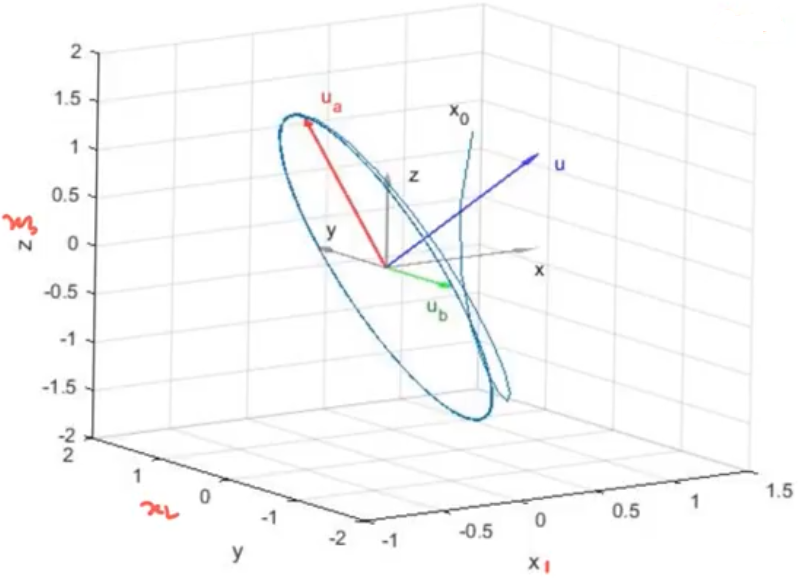
\includegraphics[width=\picwid]{traiettoria_3D_sistema_x}
\end{figure}

\subsubsection{Analisi con matrice di non semplice struttura}
17:32
